\begin{savequote}[75mm]
This is some random quote to start off the chapter.
\qauthor{Firstname lastname}
\end{savequote}

\chapter{The ATLAS detector and the Large Hadron Collider}

This chapter presents an overview of the experimental systems used to conduct the measurements presented in this thesis. First, a brief overview of the accelerator, the Large Hadron Collider, will be given. In this section, the accelerator conditions relevant to data-taking are presented as well. Next, an overview of the ATLAS experiment is given. The basics of each sub-detector's role are summarized, as well as the details of the datasets accumulated. Then, a brief interlude on the ATLAS Muon New Small Wheel upgrade is presented. While this new detector does not have a direct impact on any of the datasets taken so far, it will have an impact on future analyses and the work done on it is briefly summarized here. Finally, an overview of object reconstruction in ATLAS is given. While the details of all of the algorithms will not be presented in detail, aspects of the reconstruction performance such as object resolutions are shown as these are relevant to the two studies presented later in this thesis. 

\section{The Large Hadron Collider}

The Large Hadron Collider (LHC) is a proton-proton collider at the CERN laboratory in Geneva, Switzerland\cite{LHCPaper}. It is designed for a maximum collision center of mass energy of $\sqrt{s} = 14 \TeV$ and has a circumference of $26.7$ kilometers. Four main experiments are located at the interaction points (IP) of the accelerator: ATLAS (A Toroidal LHC ApparatuS), CMS (the Compact Muon Solenoid), ALICE (A Large Ion Collider Experiment), and LHC$b$~\cite{ATLASPaper, CMSPaper, LHCbPaper, ALICEPaper}. The studies performed in this thesis were all completed with the ATLAS detector.

Figure~\ref{fig:LHC} shows a schematic of the LHC ring and the various experiments.  

\begin{figure}[h!]
  %\vspace{20pt}
  \centering
  \captionsetup{justification=centering}

  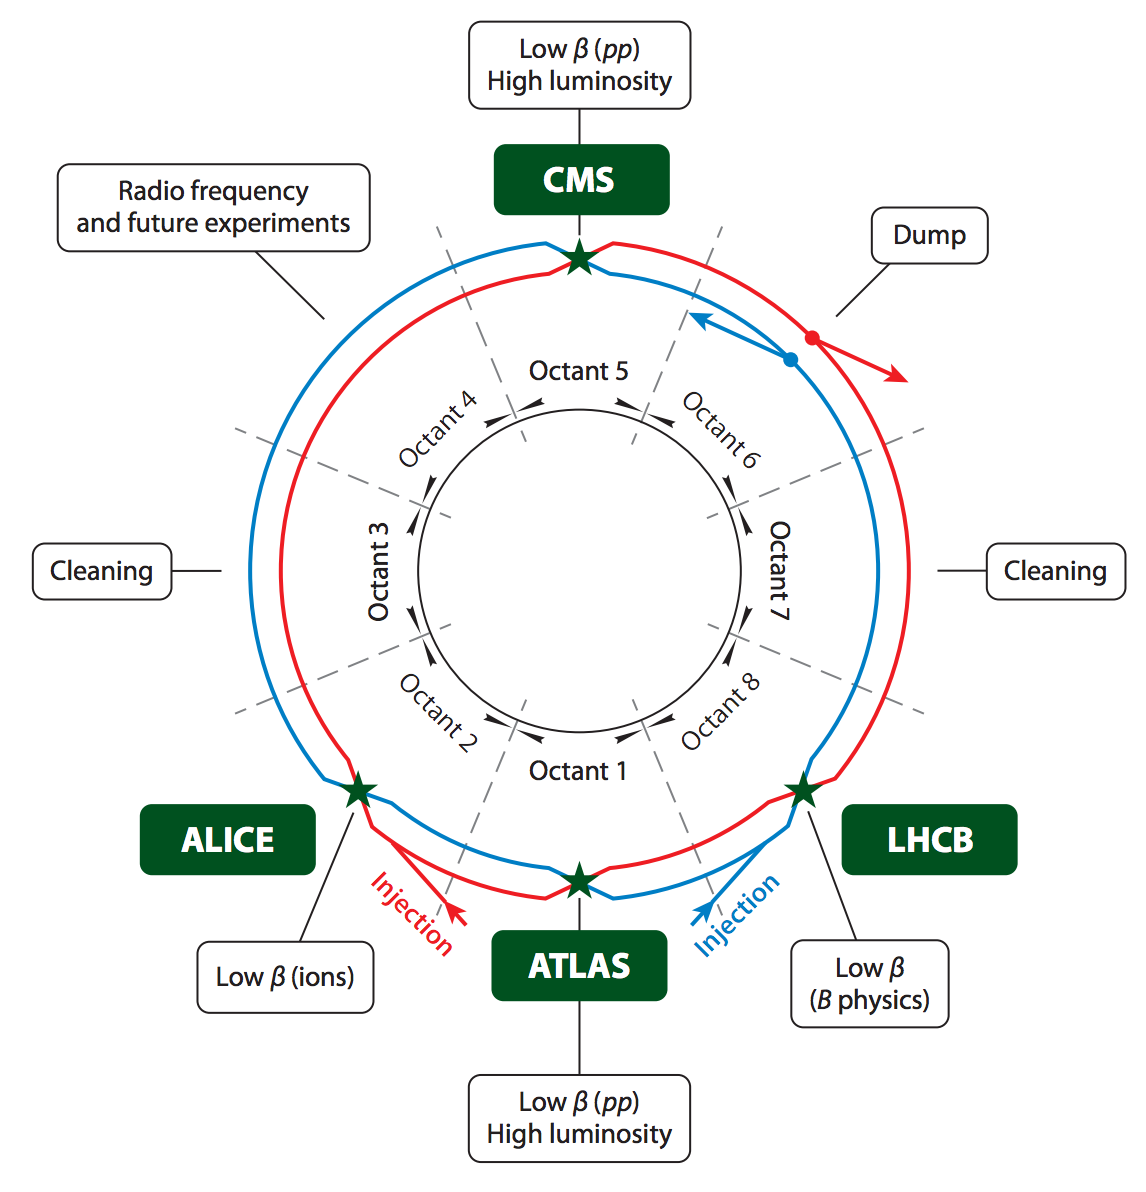
\includegraphics[width=0.7\textwidth]{figures/LHC}
   \caption{A schematic view of the LHC ring ~\cite{LHCReview}}
  \label{fig:LHC}
\end{figure}

One of the most interesting features of the LHC is in its magnet design. Because the tunnel does not have room for separate superconducting magnets for each of the beam pipes, the LHC employs a twin-bore magnet design. Each magnet must hold an $8.3$ Tesla magnetic field in order to bend the proton beams at $\sqrt{s} = 14 \TeV$. The superconducting magnets are cooled to a temperature of $1.9$ Kelvin with superfluid helium.  

\subsection{Instantaneous luminosity}

The rate of physics events expected from the accelerator is dependent on the instantaneous luminosity of the machine and the cross section of the physics process, $R_{\rm events} = L\sigma$. Here, $R_{\rm events}$ is the number of events per second, $L$ is the instantaneous luminosity of the machine, and $\sigma$ is the cross section for the physics process being measured. The instantaneous luminosity of the LHC is determined by numerous factors related to machine conditions. Equation~\ref{eqn:lumi} gives the equation for instantaneous luminosity of Gaussian beam profile~\cite{LHCReview}.

\begin{equation}
\label{eqn:lumi}
L = \frac{N_b^2 n_b f_{\rm rev} \gamma_r}{4\pi \epsilon_n \beta^*} F
\end{equation}

The LHC collides protons in bunches, and in the above equation $N_b$ is the number of protons per bunch while $n_b$ is the number of bunches per beam. Nominally, the LHC can hold up to $2808$ proton bunches. $f_{\rm rev}$ is the revolution frequency. $\epsilon_n$ is the normalized transverse beam emittance, a measurement of the average spread of the particles position-momentum space which has the dimension of length. $\beta^*$ is the value of the $beta$ function for the beam at the interaction point. It relates the emmitance to the Gaussian width of the beam with $\sigma_{\rm beam} = \sqrt{\epsilon \cdot \beta}$. $F$ is a reduction factor that corrects for the fact that the beams are colliding at an angle at the IP. 

Another way of writing the instantaneous luminosity is shown in equation~\ref{eqn:lumi2}. In this case, the instantaneous luminosity is written as the ratio of the rate of inelastic collisions with the inelastic cross section\cite{lumi-paper}. 

\begin{equation}
\label{eqn:lumi2}
L = \frac{R_{\rm inel}}{\sigma_{\rm inel}} = \frac{\mu n_b f_{\rm rev}}{\sigma_{\rm inel}}
\end{equation}

In this case, $\mu$ is the average number of interactions per bunch crossing in the accelerator. $\mu$ is a useful parameter for characterizing the amount of activity recorded in an experiment. As the instantaneous luminosity and thus $\mu$ increase, there are more interactions per bunch crossing and more activity in the detector. This is often characterized with $\langle \mu \rangle$, the measured per bunch crossing $\mu$ value averaged over all bunch crossings. The interactions inside each bunch crossing that are not the main physics process of interest are often referred to as ``pileup" interactions, and $\langle \mu \rangle$ is a measurement of the level of pileup in the detector. 

\subsection{Evolution of machine conditions}

This thesis uses datasets taken at three different center of mass energies: $\sqrt{s} = 7 \TeV$ data taken in the year $2011$, $\sqrt{s} = 8 \TeV$ data taken in the year $2012$, and $\sqrt{s} = 13 \TeV$ dataa taken in the year $2015$. In addition to increasing center of mass energy, the instananeous luminosity and parameters that determine it were evolving. Table~\ref{tab:LHC_cond} summarizes that machine conditions in each of these datasets. 

\begin{table}[h!]
\centering
\captionsetup{justification=centering}

%\begin{tabular*}{0.480\textwidth}{p{0.075\textwidth} p{0.180\textwidth} l}
\hspace{-10pt}
\begin{tabular}{|c|c|c|c|c|}
\hline
& $2011$ & $2012$ & $2015$ & Design\\ \hline
$\sqrt{s}$ [$\TeV$] & $7$ & $8$ & $13$ & $14$ \\ \hline
Number of bunches & $1380$ & $1380$ & $1825$ & $2808$ \\ \hline
Max. protons per bunch & $1.45\times10^{11}$ & $1.7\times10^{11}$ & & $1.15 \times 10^{11}$ \\ \hline
Bunch spacing [$\textrm{ns}$] & $50$ & $50$ & $25$ & $25$ \\ \hline
\specialcell{Max. instantaneous \\ luminosity [$\textrm{cm}^{-2} \textrm{s}^-1$]} & $3.7\times 10^{33}$ & $7.7\times10^{33}$ & $5\times10^{33}$ & $10^{34}$\\ \hline
$\beta^*$ [$\textrm{m}$] & $1.0$ & $0.6$ & $0.8$ & $0.55$ \\ \hline 
$\langle \mu \rangle$ & $11.6$ & $20.7$ & $13.7$ & - \\ \hline
\end{tabular}

\caption{
Evolution of LHC machine conditions~\cite{LHC_2011_2012,LHC_2015}
}
\label{tab:LHC_cond}
\end{table}


\section{The ATLAS Detector}

The ATLAS detector is a multi-purpose particle detector experiment at the LHC's Point $1$~\cite{ATLASPaper}. It has nearly $4\pi$ coverage in solid angle around the interaction point. It consists of an inner detector for measuring charged particles, electromagnetic and hadronic calorimeters, and a muon spectrometer. Figure~\ref{fig:ATLAS_overview} gives an overview of the detector.

\begin{figure}[h!]
  %\vspace{20pt}
  \centering
  \captionsetup{justification=centering}

  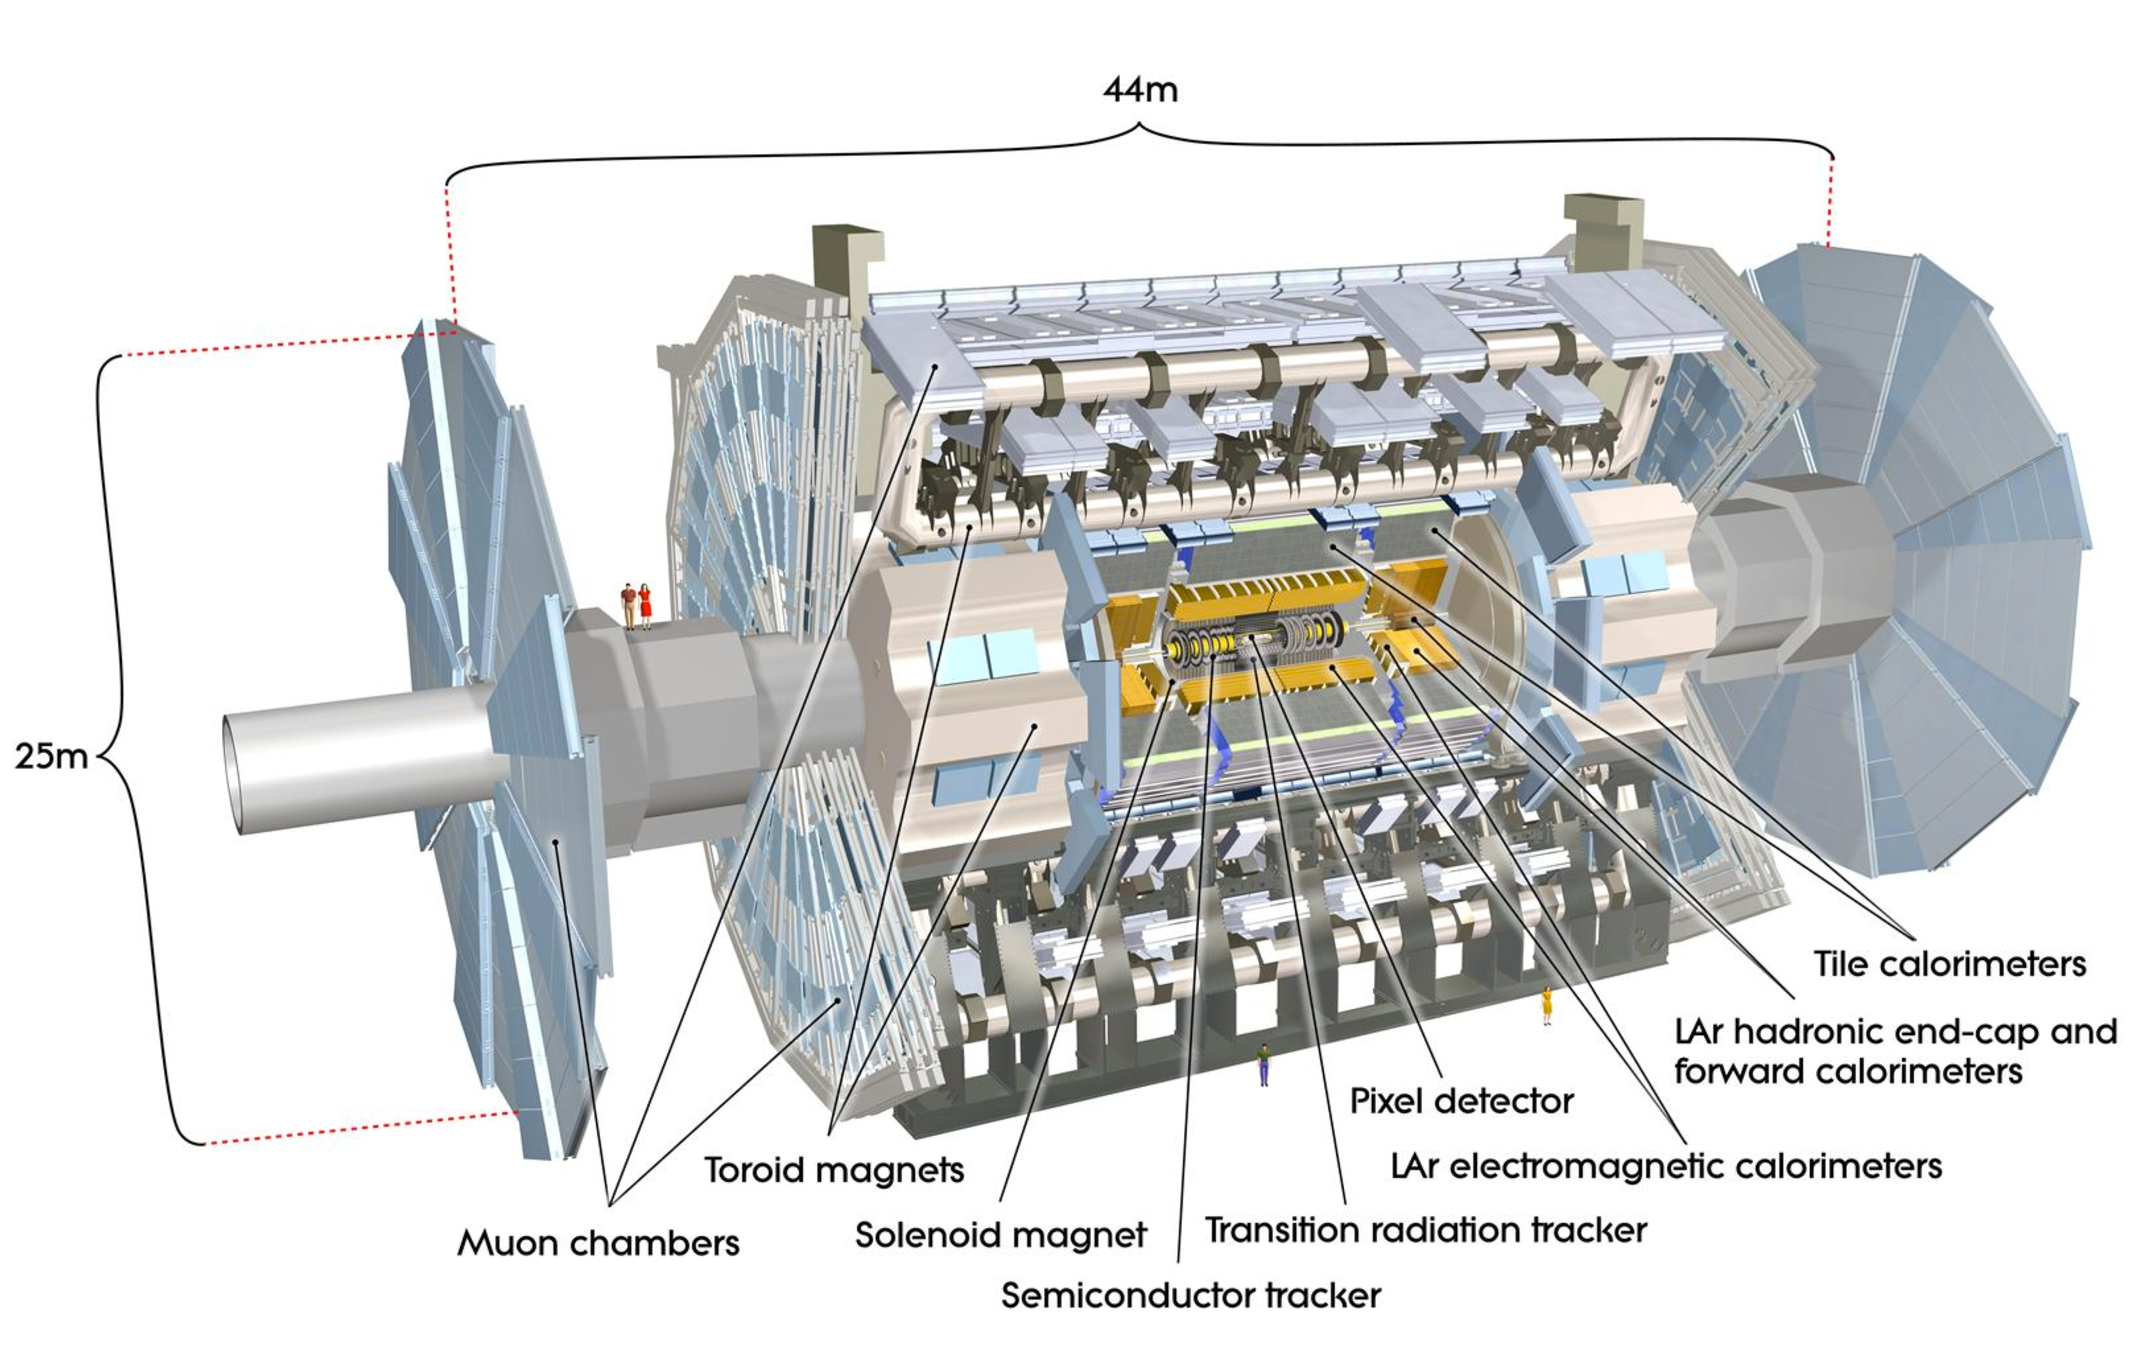
\includegraphics[width=\textwidth]{figures/ATLAS}
   \caption{A full diagram of the ATLAS detector~\cite{ATLASPaper}}
  \label{fig:ATLAS_overview}
\end{figure}

\subsection{Coordinate system}

Before defining the properties of the individual detectors, it is important to establish the coordinate system used. Figure~\ref{fig:coord} shows a schematic of the coordinate system. The azimuthal plane (perpendicular to the beam line) is defined as the $x$-$y$ plane. The angle in this plane is referred to as $\phi$. The angle relative to the beam axis is referred to as $\theta$. Rather than using $\theta$ directly as a coordinate, the experiment often uses the pseudorapidity $\eta$. $\eta$ is defined in equation~\ref{eqn:eta}. 

\begin{equation}
\label{eqn:eta}
\eta = \ln{\left(\tan\left(\frac{\theta}{2}\right)\right)}
\end{equation}

Pseudorapidity is the massless approximation of rapidity, the angle used to paramaterize boosts in special relativity. This is important for two reasons. First, it means that differences in $\eta$ are Lorentz invariant. Second, particle production is roughly constant in pseudorapidity. Particles with $\eta$ close to zero are referred to as ``central", while those at high $|\eta|$ are called ``forward". In general, two main detector topologies can be seen in figure~\ref{fig:ATLAS_overview}. There are ``barrel" elements, which surround the beam line cylindrically and are in the central region of the detector. In the forward region, there are ``endcap" regions which are arranged as disks perpendicular to the beam line. 

\begin{figure}[h!]
  %\vspace{20pt}
  \centering
  \captionsetup{justification=centering}

  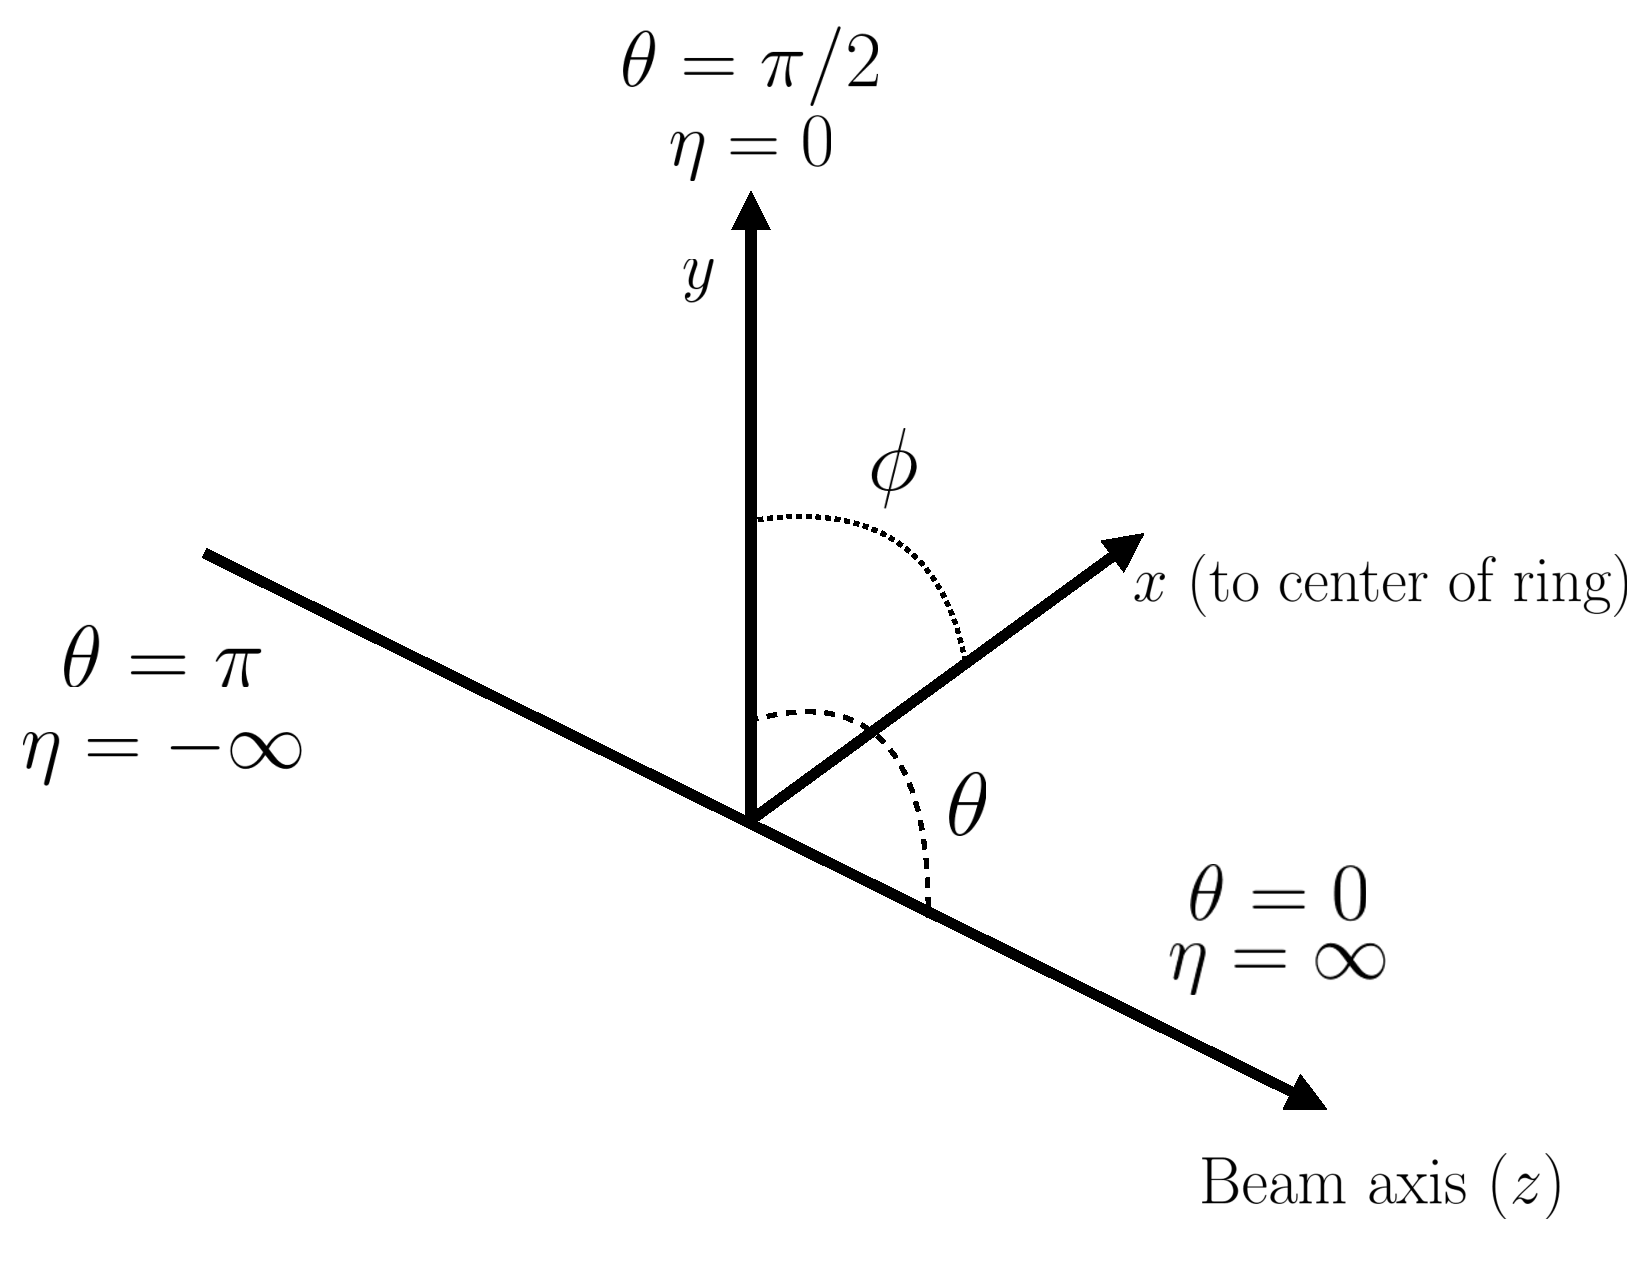
\includegraphics[width=0.8\textwidth]{figures/ATLAS_coord}
   \caption{The ATLAS coordinate system}
  \label{fig:coord}
\end{figure}

\subsection{Inner detector}

The ATLAS Inner Detector (ID) system is built for precision tracking of charged particles. It covers the range $|\eta| < 2.5$. In this range, approximately $1000$ particles are generated every bunch crossing in the detector. This requires having fine granularity to achieve the resolutions required for good momentum measurement and vertex reconstruction. 

The ID consists of three sub-components: the pixel detector, semiconductor tracker (SCT), and transition radiation tracker (TRT). It is surrounded by a solenoid providing a $2$ $\rm T$ axial magnetic field which bends particles in the transverse plane to allow for momentum measurement. Figure~\ref{fig:ID}shows the layout of each of these components. 

\begin{figure}[h!]
  %\vspace{20pt}
  \centering
  \captionsetup{justification=centering}

  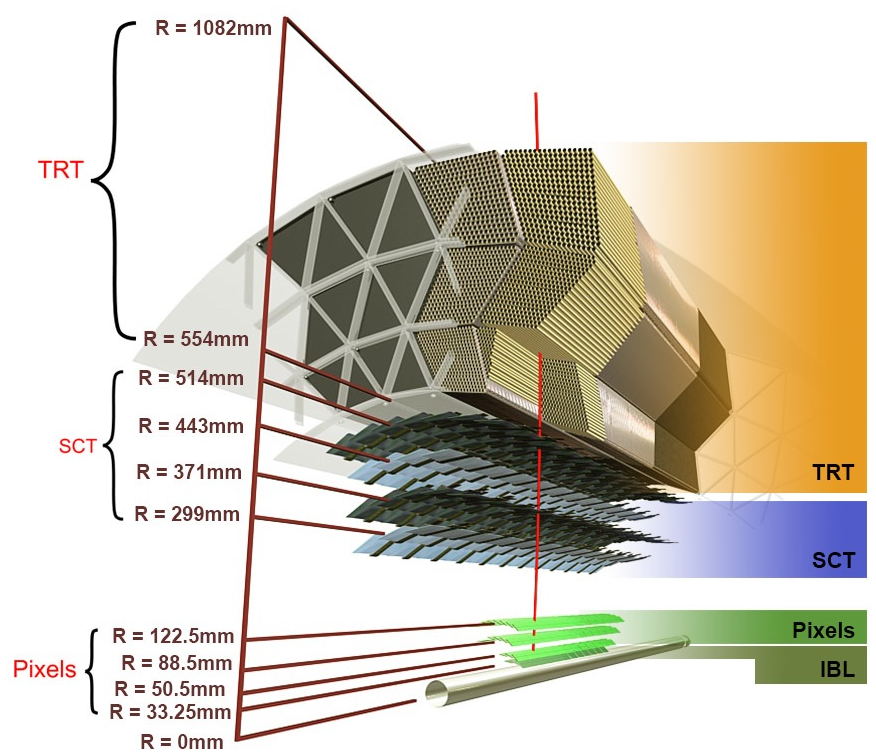
\includegraphics[width=0.7\textwidth]{figures/ATLAS_ID}
   \caption{Layout of the ATLAS Inner Detector system~\cite{Run2Tracking}}
  \label{fig:ID}
\end{figure}

\subsubsection{Pixel detector}

The pixel detector is the first detector particles traverse after being generated in proton collisions and is the most granular detector. Its operation is crucial for precision tracking and vertex reconstruction as well as higher level object reconstruction like tagging of jets from $b$-quarks. The basic sensing element in this subdetector is a silicon pixel detector. The operating principle for the silicon pixels is that of a $p$-$n$ junction. When a charged particle passes through, it creates electron-hole pairs that are then separated by the electric field. The sensors are $250\,\mu\rm m$ thick and use oxygenated $n$-type wafers with readout pixels on the $n^+$ side of the detector~\cite{ATLASPaper}. Overall, the pixel detector has $1744$ sensors and $~80.4$ million readout channels.

In the barrel region, the pixel detector has three concentric layers of sensors surrounding the beamline. In the endcap region, it consists of disks perpendicular to the beam axis. The detector is segmented in the $R$-$\phi$ plane and in $z$. Usually, three pixel layers are crossed by a charged particle track. The intrinsic accuracies of the sensors are $10\,\mu\rm m$ in $R$-$\phi$ and $115\,\mu\rm m$ in $z$ (or $R$ for the endcap).


\subsubsection{Insertable B-layer}

In Run 2, a new innermost pixel layer, known as the insertable B-layer (IBL), was added to the Inner Detector~\cite{IBL}. This layer was added to cope with the higher luminosities planned in LHC Run 2 and at the high luminosity HL-LHC. Additionaly it improves tracking position resolution which in turn improves the vertexing and $b$-tagging capabilities in ATLAS. The detector sits directly on a new beam pipe, only $33.25 \textrm{ mm}$ away from the collision points in the azimuthal plane. 

\subsubsection{Semiconductor Tracker (SCT)}

The semiconductor tracker (SCT) consists of silicon microstrips and comprises the next four layers of the ID. This sub-detector has $6.4 \textrm{cm}$ long sensors that are daisy-chained into strips with a strip pich of $80 \,\mu\rm m$~\cite{ATLASPaper}. Some of the strips have a small stereo angle to allow for measurement of both angular coordinates. In total there are $6.3$ million readout channels. The intrinsic accuracies are $17 \,\mu\rm m$ in $R$-$\phi$ and $580 \,\mu\rm m$ in $z$ (or $R$ in the endcap).

\subsubsection{Transition radiation tracker (TRT)}

The transition radiation tracker (TRT) serves two purposes. First, it consists of $4 \rm mm$ diameter straw tubes filled with a $70/27/3$\% gas mixture of xenon, carbon dioxide, and oxygen to provide tracking of charged particles. Particles typically have $36$ TRT straw tube hits per track. The material in between the straws is designed to induce transition radiation which can be useful for particle identification. As particles pass between media with different dielectric constants, they emit transition radiation that can cause additional showers in the TRT. In particular it is useful for discrimination between electrons and pions or other charged hadrons, as the amount of transition radiation is proportional to the Lorentz factor of the particle.

\subsection{Calorimeters}

The calorimeter system consists of two main sub-components: a fine granularity electromagnetic calorimeter tailored for the measurement of photons and electrons and multiple coarser hadronic calorimeters dedicated to the measurement of hadronic showers~\cite{ATLASPaper}. The calorimeter system has broader coverage than the inner detector, covering the region out to $|\eta| < 4.9$. It is also designed to deliver good containment of showers so as to limit leakage into the muon system. Figure~\ref{fig:ATLAS_calo} shows the layout of the calorimeter system. 

Both the electromagnetic and hadronic calorimeters are sampling calorimeters. They alternate active material for energy measurement with passive material for energy absorption. The materials used for each purpose vary based on the type of calorimeter and its location in the detector. 

\begin{figure}[h!]
  %\vspace{20pt}
  \centering
  \captionsetup{justification=centering}

  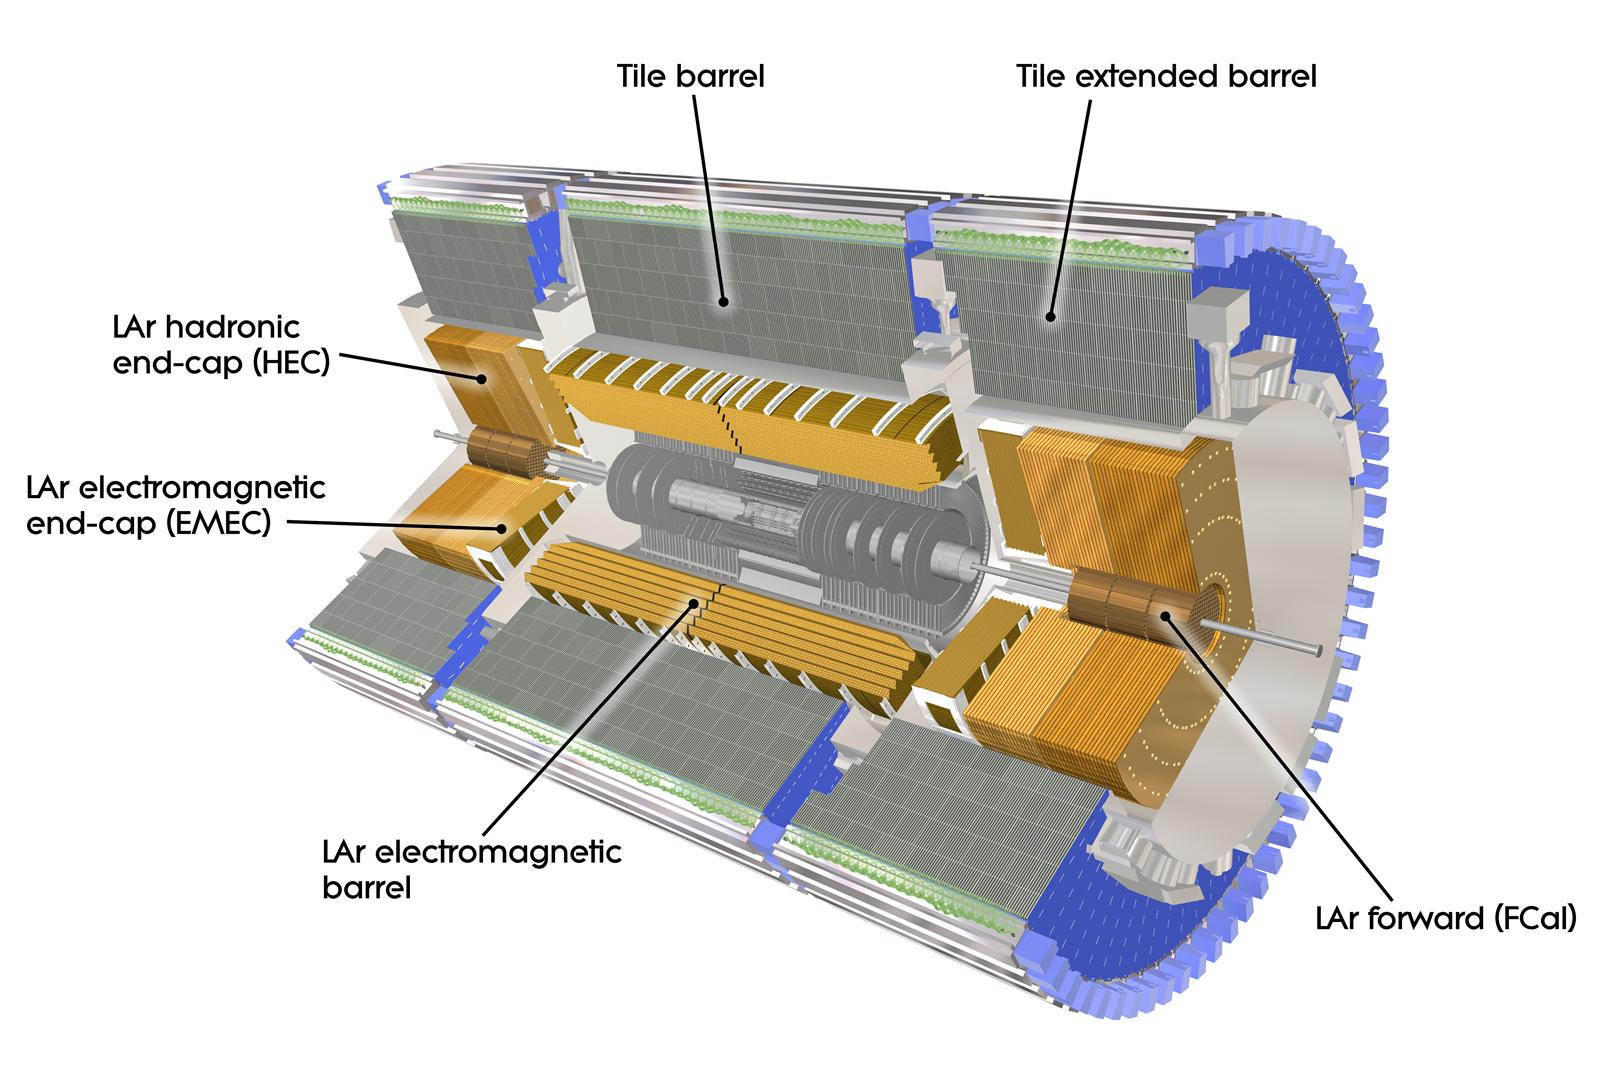
\includegraphics[width=\textwidth]{figures/ATLAS_calo}
   \caption{Layout of the ATLAS calorimeter system~\cite{ATLASPaper}}
  \label{fig:ATLAS_calo}
\end{figure}

\subsubsection{Electromagnetic calorimeter}

The electromagnetic calorimeter (EM calorimeter) use liquid Argon (LAr) as its active material and lead as its passive material. It is arrange in an accordion geometry to increase the absorption area while still allowing it to have no azimuthal cracks (complete symmetry in $\phi$). The EM calorimeter is divided into a barrel portion that extends to $|\eta| < 1.475$ and an endcap portion going from $1.375 < |\eta| < 3.2$. The region where these two units overlap is called the ``transition region". 

In order to provide good containment the calorimeter depth must be optimized. Typically, for electromagnetic calorimeters the depth is meaasured in radiation lengths. In general, the intensity of a particle beam attenuates exponentially in distance with a constant equal to the radiation length. That is, $I(x) = I_0 e^{-x/X_0}$, where $I$ is the intensity, $x$ is the distance traveled, and $X_0$ is the radiation length. The ATLAS EM calorimeter is designed to have $>22$ radiation lengths in the barrel and $> 24$ in the endcap~\cite{ATLASPaper}. 

\subsubsection{Hadronic calorimeters}

There are three types of hadronic calorimeters present in ATLAS: the tile calorimeter (TileCal), hadronic endcap (HEC), and forward calorimeter (FCal). Each one is optimized for stopping of hadronic showers and the materials chosen are specific to their placement in the detector. 

The TileCal is a scintillating tile calorimeter placed directly outside the EM calorimeter. It uses steel as the absorber and plastic scintillator tiles as the active material. It has coverage in the barrel at $|\eta| < 1.0$ and in the ``extended barrel" region of $0.8 < |\eta| < 1.7$.

The HEC had two wheels perpendicular to the beam line per endcap and is located directly behind the EM calorimeter endcap modules. The HEC covers the region from $1.5 < |\eta| < 3.2$, overlapping slightly with both the tile calorimeter and the forward calorimeter. Like the EM calorimeter, it uses liquid Argon as the active material, but it uses copper as the absorber. 

The FCal covers the most forward regions of the calorimeter system, extending to the region of $3.1 < |\eta| < 4.9$. It again uses liquid argon as its active material. For absorber, it consists of an innermost module made of copper followed by a module made of tungsten. 

The hadronic equivalent of radiation length is called the interaction length and is denoted as $\lambda$. In the barrel, the hadronic calorimeter depth is approximately $9.7\lambda$, while in the endcap is is $10\lambda$. The outer supports contribute an additional $1.3\lambda$. This is been shown to be sufficient to limit punch-through of showers to the muon system~\cite{ATLASPaper}.

\subsection{Muon spectrometer}

The muon spectrometer is dedicated to measuring the momentum and position of muons. It consists of tracking and trigger chambers which are unique in the barrel and endcap regions. The magnetic field for bending of muons is provided by a system of three large air-core toroid magnets (from which ATLAS derives its name.) These magnets provide $1.5$ to $5.5 \textrm{ Tm}$ of bending power at $0<|\eta|<1.4$ and approximately $1$ to $7.5 \textrm{ Tm}$ in the endcap region of $1.6 < |\eta| < 2.7$. The entire muon system covers the range $0 < |\eta|< 2.7$. Monitored drift tubes (MDTs) are used for tracking in the barrel and the two outer layers of the endcap, while cathode strip chambers (CSCs) are used to provide tracking in the innermost endcap wheel. In the barrel, resistive plate chambers (RPCs) are used as trigger chambers while thin gap chambers (TGCs) are used in the endcap. Figure~\ref{fig:ATLAS_muon} shows the layout of the ATLAS muon system. The entire muon system is designed with the specification of providing a $10\%$ momentum resolution for a $1 \TeV$ muon. 


\begin{figure}[h!]
  %\vspace{20pt}
  \centering
  \captionsetup{justification=centering}

  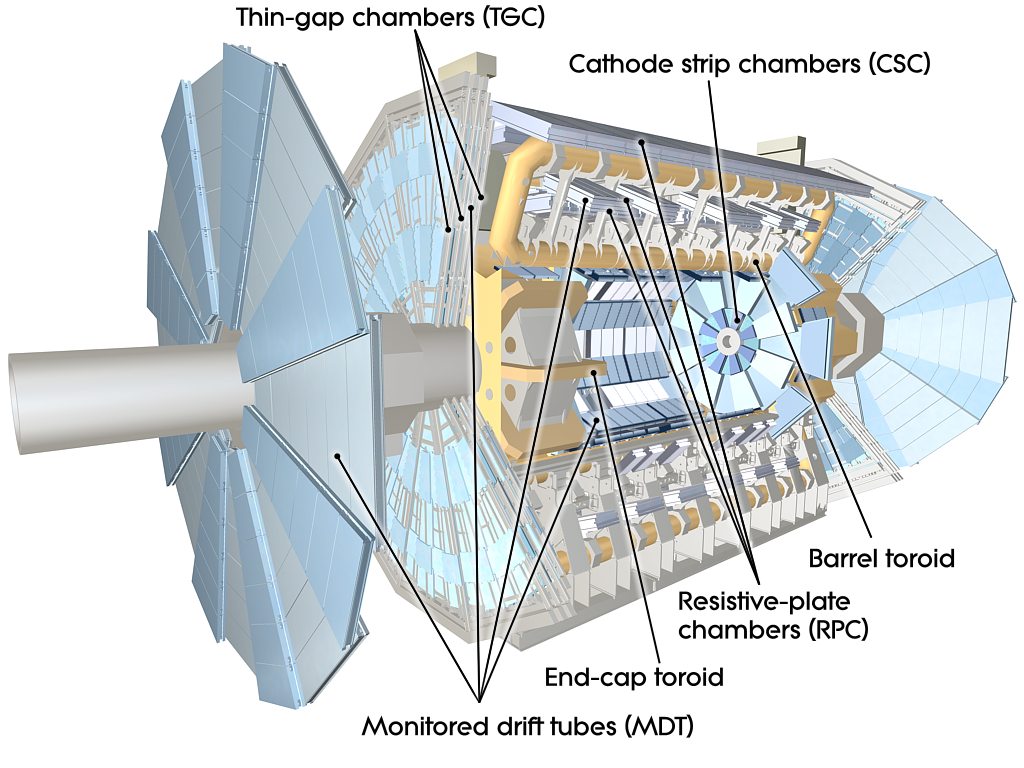
\includegraphics[width=0.9\textwidth]{figures/ATLAS_muon}
   \caption{Layout of the ATLAS muon system~\cite{ATLASPaper}}
  \label{fig:ATLAS_muon}
\end{figure}


\subsubsection{Monitored drift tubes (MDTs)}

The monitored drift tubes (MDTs) are aluminum $3 \rm cm$ diameter tubes filled with a $93/7$ \% mixture of Argon and $\textrm{CO}_2$, with trace amounts of water. As a charged particle traverses the tube, it ionizes the gas and the ions drift to a wire at the center of the tube. The radial distance of traversal of the particle in the tube is determined by the drift time of the electrons, allowing for fine position resolution. The tubes have an average resolution of $80\,\mu\textrm{m}$ per tube and a maximum drift time of approximately $700 \rm ns$. The tubes are oriented so that they give precision measurement in $\eta$ and run along $\phi$. They cover $|\eta| < 2.7$, except in the innermost layer of the endcap where they only go to $|\eta| < 2.0$~\cite{ATLASPaper}.

\subsubsection{Cathode strip chambers (CSCs)}

The cathode strip chambers cover a narrow window of the innermost endcap region at $2.0 < |\eta|< 2.7$. In this region the background rates in the cavern are particularly high and the CSCs are designed to handle these higher rates. The CSCs are multiwire proportional chambers with wires pointing in the radial direction (away from the beam pipe). The wire serves as an anode and there are two types of segmented cathode strip, one perpendicular to the wires which gives the precision measurement and one parallel which provides the transverse coordinate. It has an $80/20$ gas mixture of Argon and $\textrm{CO}_2$~\cite{ATLASPaper}. 

\subsubsection{Resistive plate chambers (RPCs)}

The resistive plate chambers (RPCs) are gaseous electrode-plate detectors covering the region $|\eta| < 1.05$. They consist of two resistive plates separated by a distance of $2\,\rm mm$. The gas mixture used is a $94.7/5/0.3$\% mixture of $\textrm{C}_2\textrm{H}_2\textrm{F}_4$, $\textrm{Iso-C}_4\textrm{H}_10$, and $\textrm{SF}_6$. It has readout strips with a pitch of $23$-$35\, \rm mm$ for both $\eta$ and $\phi$ measurement and thus provides measurement of the azimuthal coordinate in the barrel that the MDTs do not. The thin gas gap allows for a quick response time which makes it ideal for use in the trigger. There are three layers of RPCs which are referred to as the three trigger stations. They allwo for both a low $p_{T}$ and high $p_{T}$ trigger. The coincidence of hits in the innermost chambers allows for triggering of muons between $6$ and $9 \GeV$, while the outermost layer allows the trigger to select high momentum tracks in the range of $9$ to $35\GeV$~\cite{ATLASPaper}.

\subsubsection{Thin gap chambers (TGCs)}

The thin gap chambers (TGCs) are multiwire proportional chambers where the wire to cathode distance ($1.4\.\rm mm$) is smaller than the wire-to-wire distance ($1.8\,\rm mm$). They contain a gas mixture of $\textrm{CO}_2$ and $n$-pentane and use a hih electric field to gain good time resolution. They serve two functions in the end-cap system. First, they serve as the trigger chambers. Second, they also provide azimuthal coordinate measurement which the MDTs do not. They sit on the inner and middle layers of the endcap. The outermost layer's azimuthal coordinate is determined by extrapolation~\cite{ATLASPaper}.

\subsection{Magnet system}

As mentioned previously, there are two independent magnet systems in ATLAS. The first is a $2\,\rm T$ solenoid field in the inner detector which provides bending in the azimuthal plane. The second is an approximately $0.5\,\rm T$ toroidal field in the muon system which provides bending in $\eta$. Figure~\ref{fig:ATLAS_mag} shows the predicted field integral as a function of $|\eta|$~\cite{ATLASPaper}. 

\begin{figure}[h!]
  %\vspace{20pt}
  \centering
  \captionsetup{justification=centering}

   %\begin{subfigure}[t]{0.5\textwidth}
   %     \centering
   %     \includegraphics[width=0.7\textwidth]{figures/ATLAS_magnets}
   %     \caption{}
   % \end{subfigure}%
    %\begin{subfigure}[t]{0.5\textwidth}
    %    \centering
        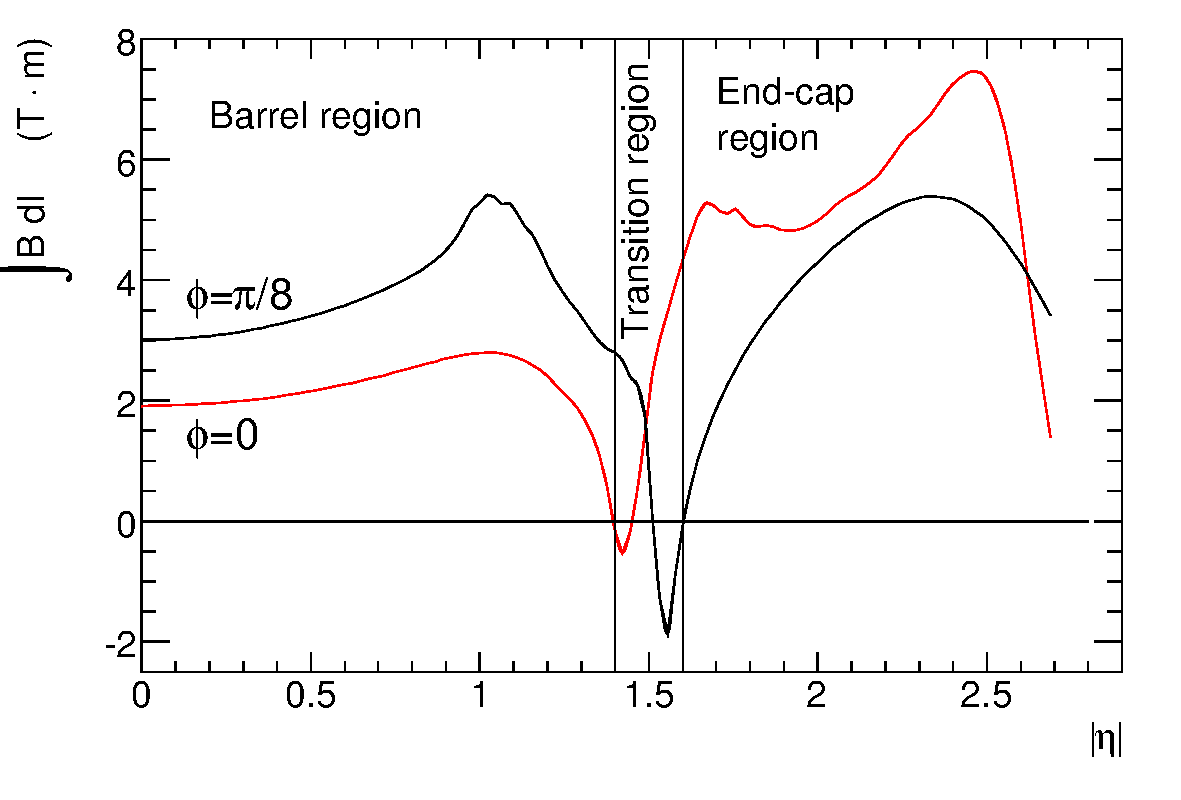
\includegraphics[width=0.6\textwidth]{figures/ATLAS_field}
    %    \caption{}
    %\end{subfigure}

   \caption{Predicted field integral as a function of $|\eta|$ for the ATLAS magnet system~\cite{ATLASPaper}}
  \label{fig:ATLAS_mag}
\end{figure}

\subsection{Trigger system}

The ATLAS trigger system searches for signatures of muons, electrons, photons, hadronically decaying $\tau$ leptons, and jets in order to save these events for further analysis. The trigger system in ATLAS is designed to reduce the maximum LHC event rate of $40\,\rm MHz$ to a more reasonable rate that can be recorded. The trigger first consists of a fast, hardware based system called the Level-$1$ (L$1$) trigger. The L$1$ trigger consists of indepdendent dedicated detector sub-components that can seed regions of interest (RoIs) for further analysis downstream. For muons, the RPCs and TGCs are used, while in the calorimeter coarsely grained sections of calorimeter cells called towers are used. Once regions of interest are seeded, a software based system called the High Level Trigger (HLT) is used to reconstruct objects and integrate information from different parts of the detector. In Run $1$ of ATLAS, the HLT consisted of two separate stages: the level $2$ (L$2$) trigger and the event filter (EF). 

The maximum trigger rate that the L$1$ trigger can handle is $75\,\rm kHz$. In the HLT, the rate of events written to disk is approximately $200\, \rm Hz$. Figure~\ref{fig:trigger_rates} shows the trigger rates for different L$1$ triggers in 2012 and 2015 for ATLAS~\cite{TriggerOps}. 

\begin{figure}[h!]
  %\vspace{20pt}
  \centering
  \captionsetup{justification=centering}

   \begin{subfigure}[t]{0.5\textwidth}
        \centering
        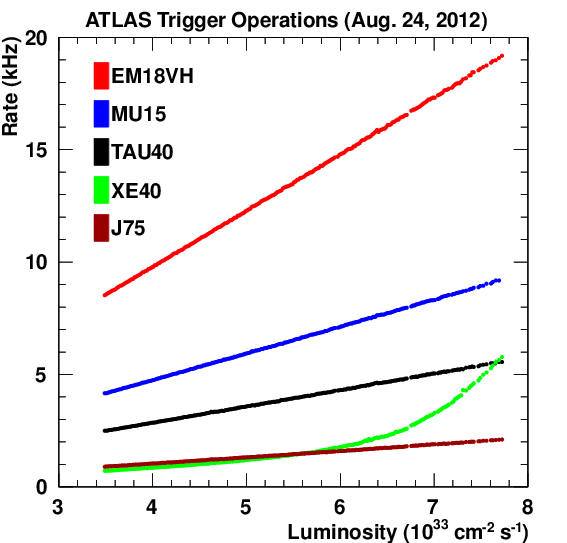
\includegraphics[width=0.7\textwidth]{figures/2012_trigger_rates}
        \caption{2012}
    \end{subfigure}%
    \begin{subfigure}[t]{0.5\textwidth}
        \centering
        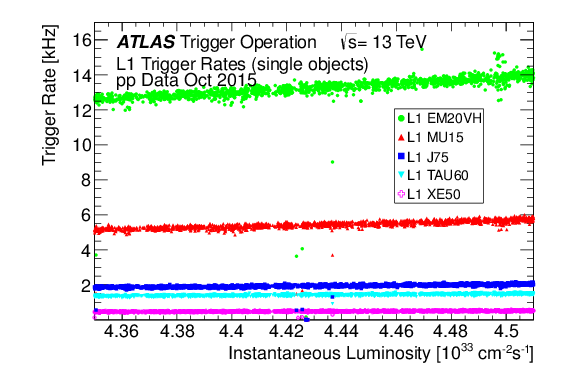
\includegraphics[width=\textwidth]{figures/2015_trigger_rate}
        \caption{2015}
    \end{subfigure}

   \caption{ATLAS trigger rates for Level-$1$ triggers as a function of instantaneous luminosity in 2012 and 2015 operation. These are single object triggers for electromagnetic clusters (EM), muons (MU), jets (J), missing energy (XE), and $\tau$ leptons (TAU). The threshold of the trigger is given in the name in $\GeV$.~\cite{TriggerOps}}
  \label{fig:trigger_rates}
\end{figure}

\subsection{ATLAS datasets}

ATLAS has collected data at center of mass energies of $7$, $8$, and $13 \TeV$. Figure~\ref{fig:lumis} shows the integrated luminosity as a function of time for each of the three collected datasets. At $\sqrt{s} = 7 \TeV$, ATLAS recorded $5.08\ifb$. Increased instantaneous luminosity in 2012 led to a larger dataset of $21.3 \ifb$ recorded at $\sqrt{s} = 8 \TeV$. After Long Shutdown $1$ (LS$1$) of the LHC and a restart in 2015, ATLAS recorded $3.9\ifb$ of data at $\sqrt{s} = 13 \TeV$. ~\cite{Lumi_Run1, Lumi_Run2} 

\begin{figure}[h!]
  %\vspace{20pt}
  \centering
  \captionsetup{justification=centering}

   \begin{subfigure}[t]{0.5\textwidth}
        \centering
        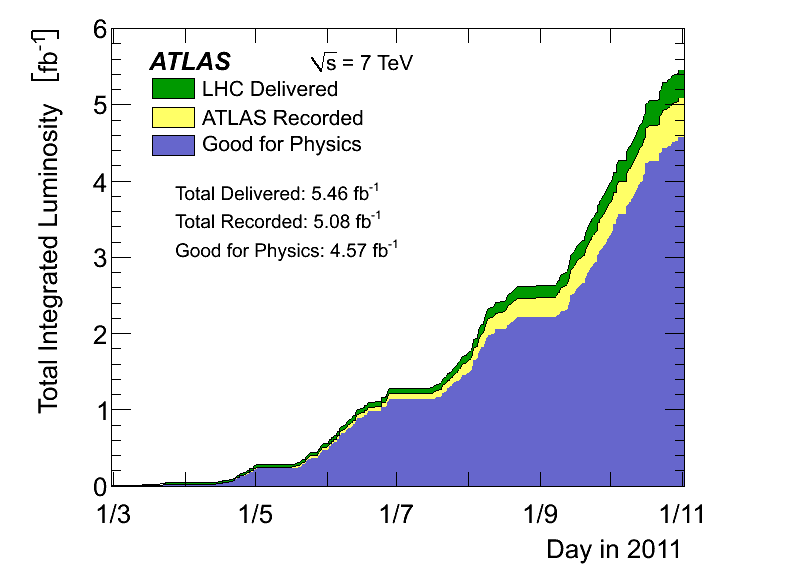
\includegraphics[width=\textwidth]{figures/ATLAS_lumi_2011}
        \caption{$\sqrt{s} = 7 \TeV$ (2011)}
    \end{subfigure}%
    \begin{subfigure}[t]{0.5\textwidth}
        \centering
        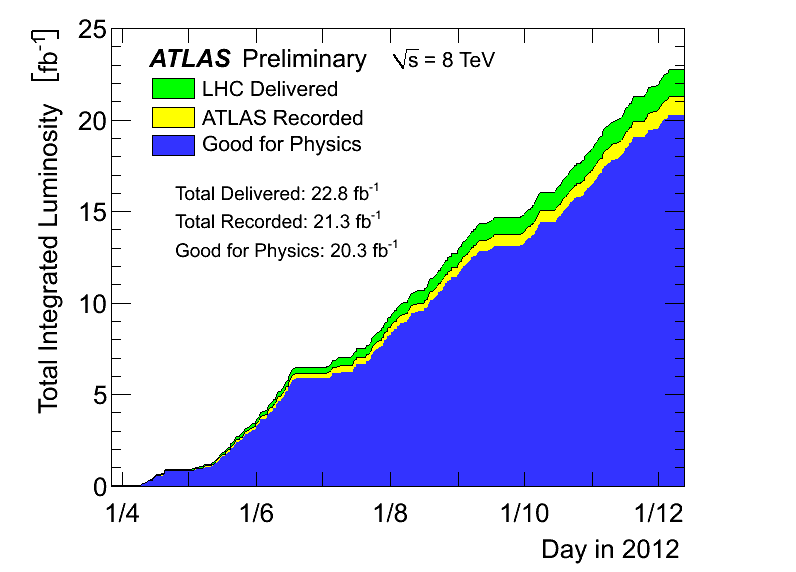
\includegraphics[width=\textwidth]{figures/ATLAS_lumi_2012}
        \caption{$\sqrt{s} = 8 \TeV$ (2012)}
    \end{subfigure}
    \begin{subfigure}[t]{0.5\textwidth}
        \centering
        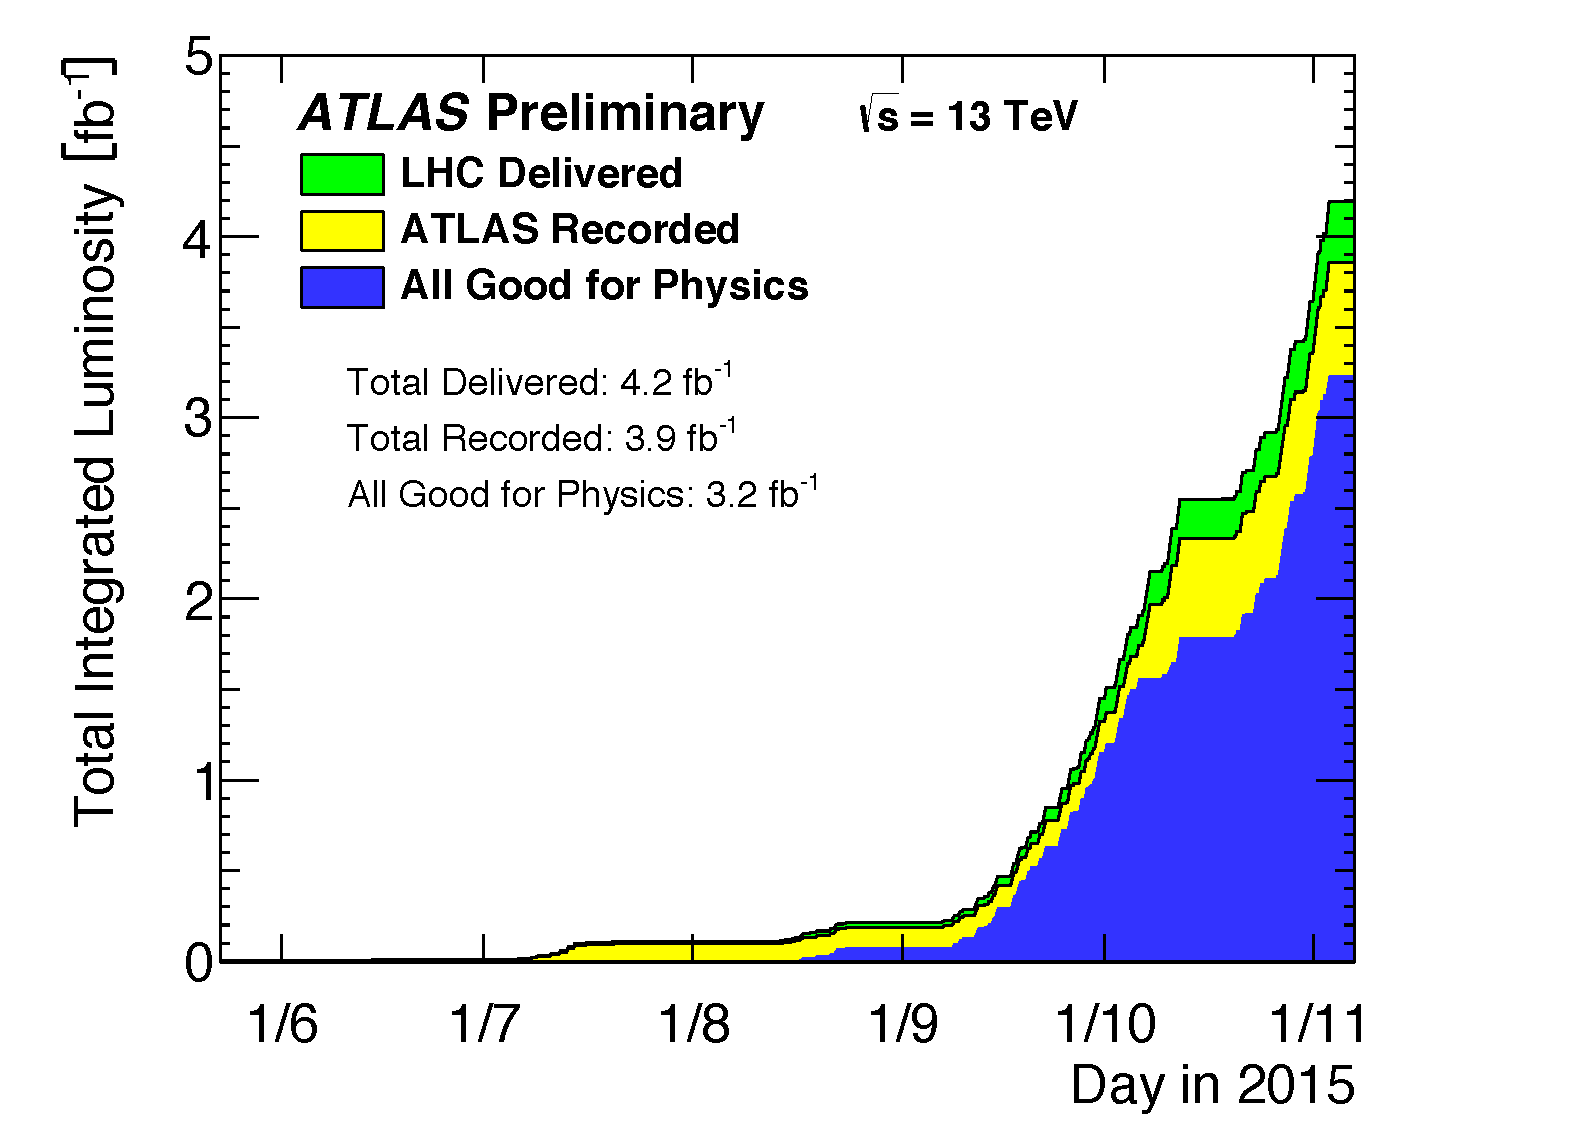
\includegraphics[width=\textwidth]{figures/ATLAS_lumi_2015}
        \caption{$\sqrt{s} = 13 \TeV$ (2015)}
    \end{subfigure}

   \caption{Instantaneous luminosity as a function of time for data recorded by ATLAS at different center of mass energies~\cite{Lumi_Run1, Lumi_Run2}}
  \label{fig:lumis}
\end{figure}


\section{The ATLAS Muon New Small Wheel Upgrade}

As the LHC continues operation, it is scheduled to be upgraded in several phases to allow it to reach higher instantaneous luminosities and thus collect larger datasets. These conditions will open new doors for study of rare physics processes but will also present interesting challenges that must be faced. ATLAS will require new detector technologies to cope with the increased background rates in the cavern in these high luminosity conditions. One such upgrade, scheduled to be installed during Long Shutdown $2$ (LS$2$) of the LHC in 2018, is the ATLAS Muon New Small Wheel (NSW) upgrade~\cite{NSW_TDR}. The NSW will replace the innermost end-cap wheel of the muon system with new technologies, as this is the part of the muon detector closest to the beam and thus suffers from the highest rates. 

\subsection{Motivation}

The motivation of the NSW is two-fold. First, the objective is to alleviate the decreased tracking efficiency that comes in a high rate environment. As figure~\ref{fig:mdt_hit_rate}, at the LHC design luminosity both the efficiency of recording hits and reconstructing track segments in the MDTs decreases at the LHC design luminosity. 

\begin{figure}[h!]
  %\vspace{20pt}
  \centering
  \captionsetup{justification=centering}

  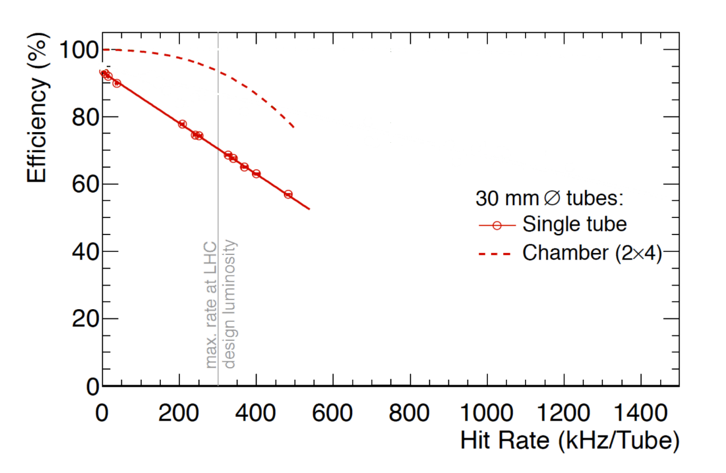
\includegraphics[width=0.7\textwidth]{figures/MDT_hit_rate}
   \caption{MDT tube hit (solid) and segment (dashed) efficiency as a function of hit rate per tube~\cite{NSW_TDR}}
  \label{fig:mdt_hit_rate}
\end{figure}

Second, the NSW will work to alleviate the rate of fake triggers arising in the endcap. Figure~\ref{fig:NSW_trig} shows the extrapolated trigger rates as a function of the $p_{T}$ threshold with and without the NSW upgrade. As the figure shows, the NSW upgrade will reduce the trigger rate by an order of magnitude compared to the current endcap trigger system. 

\begin{figure}[h!]
  %\vspace{20pt}
  \centering
  \captionsetup{justification=centering}

  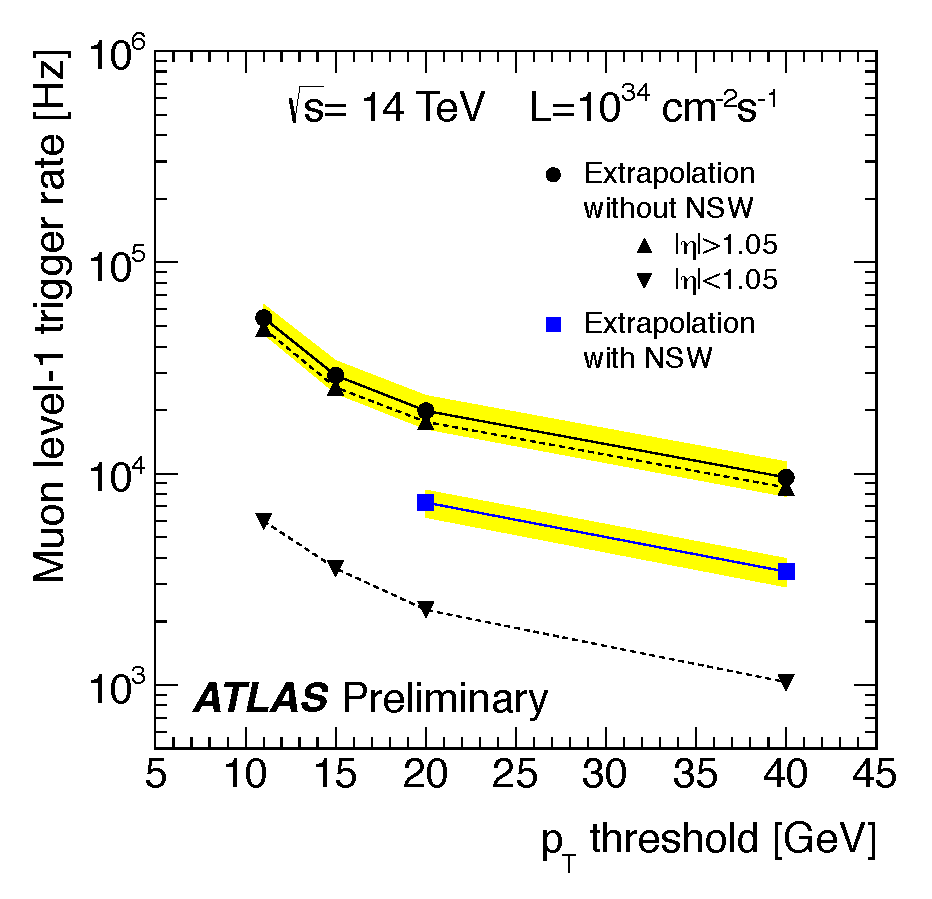
\includegraphics[width=0.7\textwidth]{figures/NSW_trigger_rate}
   \caption{Trigger rate as a function of $p_{T}$ threshold with and without the NSW upgrade~\cite{NSW_TDR}}
  \label{fig:NSW_trig}
\end{figure}

\subsection{Physics Impact}

Maintaining low $p_{T}$ thresholds for muons while still staying within the trigger rate budget at Level $1$ ($20\,\textrm{kHz}$) for the muon system is crucial for physics analyses to be successful in high luminosity conditions. One realm where the lepton trigger threshold is especially important is in Higgs physics. In the $\HWW$ analysis, one of the $W$ bosons is off shell and tends to decay to soft leptons. In associated production of a Higgs with a $W$, the lepton is also important because the lepton provides the main handle which allows the event to be triggered. Table~\ref{tab:NSW_trig_efficiencies} shows the impact of increasing the trigger thresholds on these analyses. It shows that either raising the threshold or using only the barrel both have significant impacts on the signal efficiency. With the NSW, the signal efficiency is largely maintained and the triggers can be unprescaled.

\begin{table}[h!]
\centering
\captionsetup{justification=centering}

%\begin{tabular*}{0.480\textwidth}{p{0.075\textwidth} p{0.180\textwidth} l}
\hspace{-10pt}
\begin{tabular}{|c|c|c|}
\hline
Threshold & $H\to b\bar{b}$(\%) & $\HWW$ \\ \hline
$p_{T} > 20 \GeV$ & $93$ & $94$ \\ \hline
$p_{T} > 40 \GeV$ & $61$ & $75$ \\ \hline
$p_{T} > 20 \GeV$ (barrel only) & $43$ & $72$ \\ \hline
$p_{T} > 20 \GeV$ (with NSW) & $90$ & $92$ \\ \hline
\end{tabular}

\caption{
Signal efficiencies for $WH$ production with $H\to b\bar{b}$ and $H\to WW^* \to \mu \nu qq$ under different trigger configurations~\cite{NSW_TDR}.
}
\label{tab:NSW_trig_efficiencies}
\end{table}


\subsection{Detector technologies}

\subsection{Micromegas trigger}

\section{Object Reconstruction in ATLAS}
